\section{Beam diagnostic at ESS}

\begin{frame}
  \frametitle{Beam diagnostic at ESS}
  \begin{block}{Eye of the accelerator}
    \begin{itemize}
      \item
    \end{itemize}
  \end{block}
  \begin{block}{Various type of information}
    \begin{itemize}
      \item
    \end{itemize}
  \end{block}
  \begin{block}{Transverse profile measurement}
    \begin{itemize}
      \item
    \end{itemize}
  \end{block}
\end{frame}

\begin{frame}
  \frametitle{Profile measurement method}
  \begin{columns}
    \begin{column}{0.45\textwidth}
      \begin{block}{Wire Scanner/SEM Grid}
        Measurement of the secondaries electrons or hadronic cascade emitted during the collision of proton with one or more wires.
      \end{block}
      \begin{block}{Pro/cons}
        \begin{itemize}
          \item
        \end{itemize}
      \end{block}
    \end{column}
    \begin{column}{0.45\textwidth}
      Image/Schema
      \begin{block}{Use at ESS}
        \begin{itemize}
          \item Everywhere
          \item But low duty cycle
        \end{itemize}
      \end{block}
    \end{column}
  \end{columns}
\end{frame}

\begin{frame}
  \frametitle{Profile measurement method}
  \begin{columns}
    \begin{column}{0.45\textwidth}
      \begin{block}{FPM}
        Measurement of the fluorescence induced by the beam.
      \end{block}
      \begin{block}{Pro/cons}
        \begin{itemize}
          \item
        \end{itemize}
      \end{block}
    \end{column}
    \begin{column}{0.45\textwidth}
      Image/Schema
      \begin{block}{Use at ESS}
        \begin{itemize}
          \item In the hot parts of the accelerator
          \item At low duty cycle
        \end{itemize}
      \end{block}
    \end{column}
  \end{columns}
\end{frame}

\begin{frame}
  \frametitle{IPM}
  \begin{columns}
    \begin{column}{0.45\textwidth}
      \begin{block}{How it works}
        \begin{enumerate}
          \item Beam protons pass through the residual gas, inducing ionizations: $e^-$/ion pairs.
          \item An electric field drives $e^-$ or ions towards a segmented readout system.
          \item Profile in one transverse direction. Complete profile: pair of IPMs.
        \end{enumerate}      
      \end{block}
    \end{column}
    \begin{column}{0.45\textwidth}
      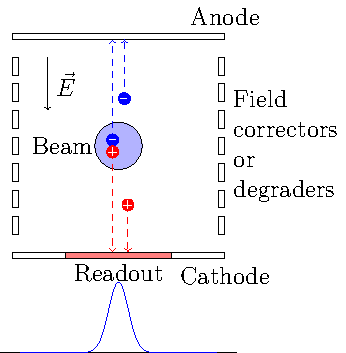
\includegraphics[width=\textwidth]{02_ESS/fig/fig000_IPM.pdf}
    \end{column}
  \end{columns}
\end{frame}

\begin{frame}
  \frametitle{IPM}

\end{frame}